\section{Practical Application}
%\lipsum[1-2]
We wanted to find remaining traces in memory from communication data and application metadata. For this we used the phone Sony Xperia M2 with Android 5.1.1. The phone has 1GB of RAM.

\subsection{Laboratory Environment}
The phone was factory reset to ensure a reproducible result. At this point the phone was rooted using the KingRoot application version 4.9.5. This process did not require restart of the phone, potentially leaving traces of memory from before rooting and making it ideal for memory forensics provided the phone can be unlocked regardless of root status. After testing the root, the phone was restarted to ensure a consistent state. As part of this process ADB USB debugging was enabled. A memory cleaning app 'Clean Master'(version 5.14.4) was installed which claimed to remove temporary files and free memory.\\\\ %TODO: Write about usafe of this application in the appropriate sections
We used this tool because we wanted to check if data could survive a cleaning tool. Since we could not test over longer periods of time, and since the phone had very low memory, we used a cleaning tool to mimic an environment for safety conscious users. Based on what discussed in the section \ref{background} about phone memory, it would be possible to get more data from the memory dump with a phone with more memory space than 1GB. The average phone today have around 4GB of memory and would possibly provide us with more data and more data over a longer time period.\\\\Several applications was installed for testing. The applications installed were:
\begin{description}
\begin{itemize}
\item{Facebook}
\item{Facebook Messenger}
\item{Snapchat}
\item{WhatsApp}
\item{Jodel}
\item{Google Apps}
\begin{itemize}
\item{Preinstalled on the phone, including GMail, Maps and Chrome} %TODO: The phone came with ... installed?
\end{itemize}
\end{itemize}
\end{description}
Since this was performed after rooting of the phone, testing of remains in memory when rooting was impossible. Github was accessed using the Chrome browser.
%Some services were accessed using the Chrome browser:
%\begin{description}
%\item[GitHub]
%\end{description}
\subsection{Process} %TODO: Bedre navn
This section outlines the steps used for preparing the services and applications for memory forensics.

\subsubsection{Creation of credentials}
We created user accounts corresponding to individual applications. A full list is found in table \ref{tbl:credentials}.\\
\begin{table}
\begin{tabular}{l|l|l}
Service & User Name & Password \\ 
\hline 
Facebook & mis2016forensics@gmail.com & hackmyphone01 \\ 
Snapchat & canuhackmyphone & hackmyphone07 \\ 
WhatsApp & [Phone number] & - \\ 
Google & mis2016forensics@gmail.com & hackmyphone \\ 
Github & canuHackmyphone & hackmyphone06 \\ 
\end{tabular} 
\caption{Credentials used}
\label{tbl:credentials}
\end{table}

The credentials for WhatsApp has been removed from the list, however a normal phone number was used, together with a password.

After creation of the accounts in the applications, the account was used to authenticate with the applications.
% Create User accounts
% Log in to user accounts

\subsubsection{Creating searchable data}
In each of the applications, a normal session was fabricated with easily searchable data.
The types of data used for each application is specified below:
\begin{description}
\item[Facebook] \hfill\\
Information about user and friends.
\item[Facebook messenger]\hfill\\
Unique random strings and images from camera taken in application.
\item[Snapchat]\hfill\\
Images from camera taken in application.
\item[WhatsApp]\hfill\\
Unique strings and images from camera taken in application.
\item[GMail]\hfill\\
Unique random strings and images from camera taken in application.
\item[Google Chrome]\hfill\\
Credentials to GitHub. Web history.
\item[Google Maps]\hfill\\
GPS data, locations and route between locations.
\item[Jodel]\hfill\\
Unique string and image from camera taken in application.
\end{description}
In addition to the data listed, credentials as stored by the application is present.

\begin{figure}[h]
\centering
 \begin{subfigure}[b]{0.15\textwidth}
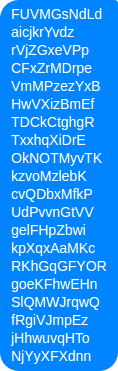
\includegraphics[width=\textwidth]{figures/messenger_string}
\caption{Messenger}
\end{subfigure}
 \begin{subfigure}[b]{0.2\textwidth}
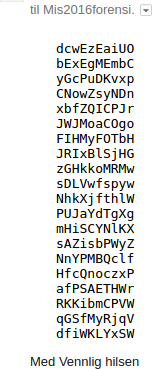
\includegraphics[width=\textwidth]{figures/random_string_in_gmail}
\caption{GMail}
\end{subfigure}
\caption{Example of string used}
\end{figure}
% Send messages using the apps
% Receive messages

% Strings used
% Use of graphic images



\subsubsection{Extracting memory}
To extract the memory AMExtractor\cite{yang2016tool} was chosen.
 It did not have a profile for the phone, so a profile for extraction method, size of the memory page structure and memory model was created and tested. It was determined that the phone had a 32 byte memory page structure, which Yang\cite{yang2016tool} claims is a typical size. The memory model was flat, which meant that it was contiguous making it simpler to copy.
 
 The tool was then compiled using the ndk-build tool which is part of the Android SDK. The local kernel headers on the machine used to compile was different from the ones used in the AMExtractor and thus a definition for the data type had to be added from an older version of the header file.
 
 The phone was then connected using ADB and the AMExtractor binary for the CPU architecture of the phone(armeabi-v7a), was copied to the phone using 'adb push'. The binary was pushed to the /data/local/tmp/ directory. A shell session was then initiated using adb shell. Inside the shell the following commands were executed to elevate privileges and test AMExtractor:
 \begin{lstlisting}[language=bash]
# su
# cd /data/local/tmp/
# chmod 755 ./AMExtractor
# ./AMExtractor
# dmesg | tail
 \end{lstlisting}
 In the kernel log a few entries had been added by AMExtractor indicating success.
 
 Next the memory dump was prepared using:
  \begin{lstlisting}[language=bash]
# ./AMExtractor -d
 \end{lstlisting}
 
AMExtractor dumps the memory to a port on localhost. To get the dump off the phone the port was forwarded over ADB with 
 \begin{lstlisting}[language=bash]
# adb forward tcp:31415 tcp:31415
 \end{lstlisting}
Next the memory dump was started with
 \begin{lstlisting}[language=bash]
# nc 127.0.0.1 31415 > dump
  \end{lstlisting}

After the memory dump had been performed, the file size was checked to ensure it matched the memory size of the phone.

\subsubsection{Searching memory}
The extracted memory was searched using the credentials from table\ref{tbl:credentials} and strings which was previously entered. For this purpose the 'strings' tool was used to extract continuous regions of ASCII text and 'grep' was used to search in this text. This has the disadvantage of only finding continuous buffers using simple storage mechanisms, but is quick to execute.

\subsubsection{Carving memory}
To find other types of resources a simple file carving was attempted using 'scalpel' with matches for the following file types:
\begin{itemize}
	\item PNG
	\item JPG
	\item TIFF
\end{itemize}
